

%\subsection{Alternative to DGLAP DIS models}
Different approaches that are alternatives to the DGLAP formalism can be used to analyse DIS data in \fitter.
These include several different dipole models and the use of 
transverse momentum dependent, or unintegrated PDFs, uPDFs.
These approaches are discussed below.

\subsection{DIPOLE models}

The dipole picture provides an alternative approach to virtual photon-proton
 scattering at low $x$ which allows the description of both inclusive and 
diffractive processes.
 In this approach, the virtual photon fluctuates into a $q\bar q$ (or $q\bar q g$) 
 dipole which interacts with the proton~\cite{NNZ:91}.  
The dipoles can be viewed as quasi-stable quantum mechanical states, which have very long 
life time $\propto 1/m_p x\;$ and a size which is not changed by scattering.
%A schematic view of dipole factorisation at small $x$ in DIS is illustrated in figure~\ref{fig:dipole}.
The dynamics of the interaction are embedded in the dipole scattering amplitude.

%\begin{figure}
%\begin{center}
%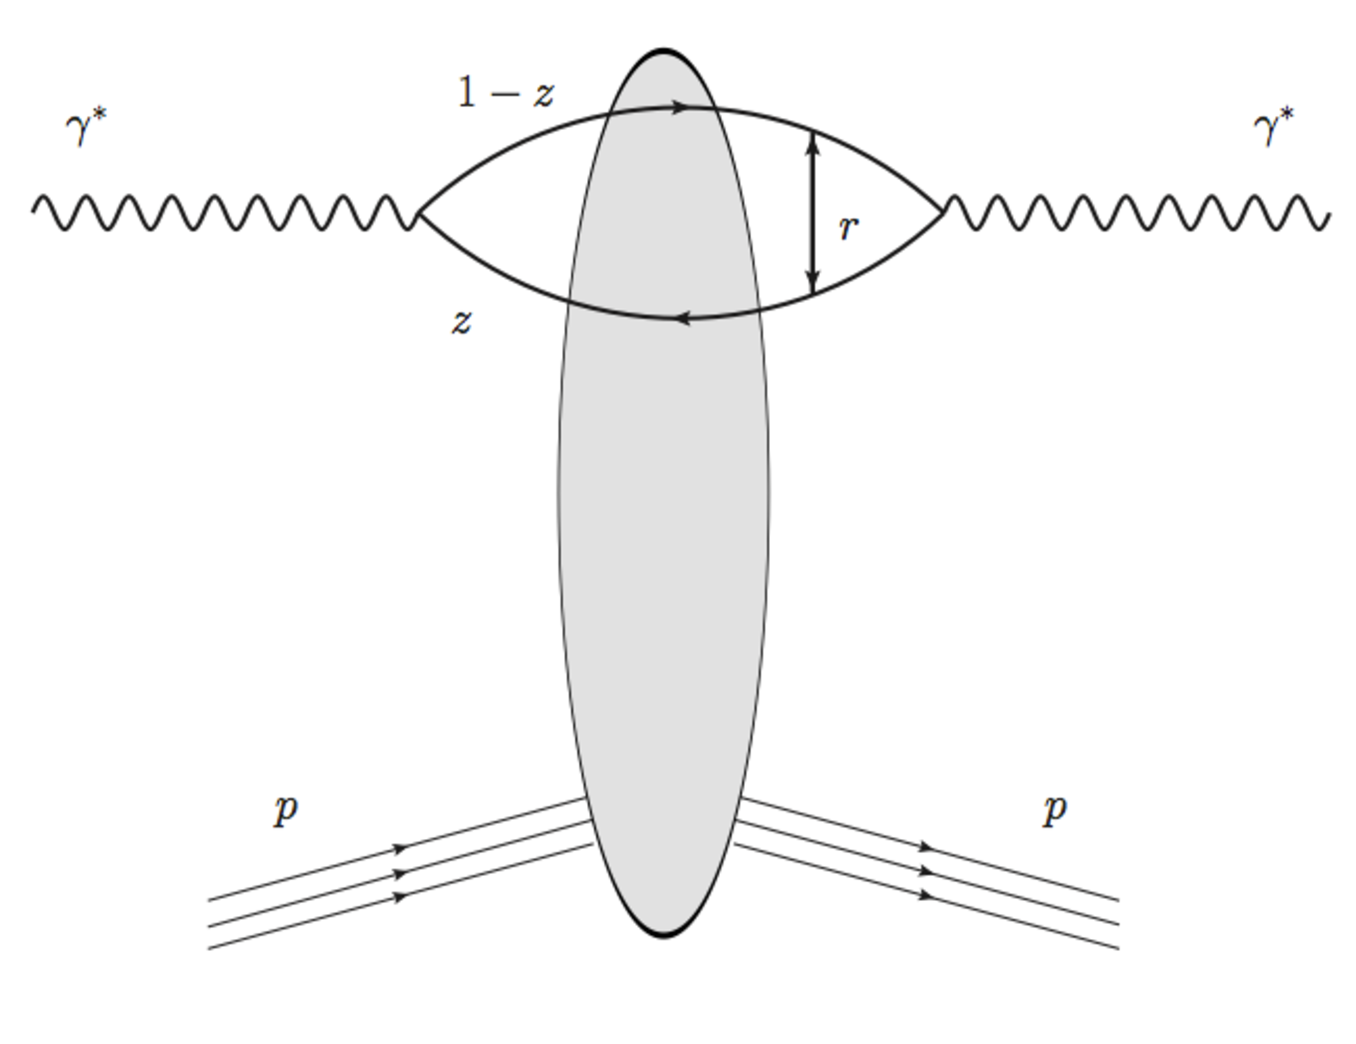
\includegraphics[width=0.5\linewidth]{figures/dipole.pdf}
%\end{center}
%\caption{Schematic diagram of dipole factorisation for the inclusive cross section in DIS.}
%\label{fig:dipole}
%\end{figure}

Several dipole models which assume different behavior of the dipole-proton 
cross sections are implemented in \fitter:
%\begin{itemize}
%\item the original Golec-Biernat-W\"usthoff (GBW)~\cite{Golec-Biernat:1998js} 
the Golec-Biernat-W\"usthoff (GBW)
dipole saturation model~\cite{Golec-Biernat:1998js},
the colour glass condensate approach to the high parton density 
regime called the Iancu-Itakura-Munier (IIM) dipole model~\cite{Iancu:2003ge} and 
a modified GBW model which takes into account the effects of  
DGLAP evolution called the Bartels-Golec-Kowalski (BGK) dipole model~\cite{Bartels:2002cj}.
%\end{itemize}

\begin{description}
\item \bf {GBW model:} \rm
In the GBW model the dipole-proton cross section $\sigma_{\text{dip}}$ is given by
\begin{equation}
\label{eGBW}
   \sigma_{\text{dip}}(x,r^{2}) = \sigma_{0} \left(1 - \exp \left[-\frac{r^{2}}{4R_{0}^{2}(x)} \right]\right),
\end{equation}
where $r$ corresponds to the transverse separation between the quark and the antiquark, and $R_{0}^{2}$
 is 
%an $x$ dependent scale parameter, having the form $R_{0}^{2}(x)=\left(x/x_{0}\right)^{\lambda}$.
an $x$-dependent scale parameter which represents the spacing of the gluons in the proton. $R_{0}^{2}(x)=\left(x/x_{0}\right)^{\lambda}$ is called the saturation radius.
The fitted parameters are the cross-section normalisation $\sigma_{0}$ and $x_{0}$ and $\lambda$. This model gives exact Bjorken scaling when the dipole size $r$ is small.
%%%%

\vspace{0.1cm}
\item \bf {IIM model:} \rm
The IIM model assumes an improved expression for the dipole cross section which is based on the 
Balitsky-Kovchegov equation~\cite{Balitsky:1995ub}. The explicit formula for $\sigma_{\text{dip}}$ 
can be found in~\cite{Iancu:2003ge}. The fitted parameters are an alternative scale parameter $\tilde{R}$, $x_{0}$ and $\lambda$.
%%%%

\vspace{0.1cm}
\item \bf {BGK model:} \rm
The BGK model modifies the GBW model by taking into account the  DGLAP evolution
of the gluon density. 
The dipole cross section is given by
\begin{equation}
\begin{array}{lcl}
   \sigma_{\text{dip}}(x,r^{2})  =  \sigma_{0} 
\left(1 - \exp \left[-\frac{\pi^{2} r^{2} \as (\mu^{2}) xg(x,\mu^{2})}{3 \sigma_{0}} \right]\right).
\end{array}
\label{eBGK}
\end{equation}
The factorization scale $\mu^{2}$ has the form $\mu^{2} = C_{bgk}/r^{2}+\mu^{2}_{0}$.
%This model uses the following gluon density at the starting scale $Q_{0}^{2}=1\mbox{ GeV}^{2}$.
This model relates to the GBW model using the idea that the spacing $R_0$ is inverse to the gluon density.
The gluon density parametrized at some starting scale $Q_{0}^{2}$ by Eq.~\ref{eqn:pdf_std}
%$ xg(x) = A_{g} x^{-\lambda_{g}}(1-x)^{C_{g}} $
is evolved to larger scales using DGLAP evolution.
The fitted parameters for this model are $\sigma_{0}$, $\mu^{2}_{0}$ and three parameters for the gluon density: $A_{g}$, $\lambda_{g}$, $C_{g}$. The parameter $C_{bgk}$ is fixed: $C_{bgk} = 4.0$. 
%%%%

\vspace{0.1cm}
\item \bf {BGK model with valence quarks:} \rm

The dipole models are valid in the low-$x$ region only, where the valence quark contribution is small.
%, of the order of 5\%. 
The new HERA $F_2$ data have a precision which is  better than 2$\%$. Therefore, in \fitter the contribution of the valence quarks can be taken from the PDF fits and added to the original 
BGK model \cite{Belov,Luszczak:2013rxa}, this is uniquely possible within the \fitter framework.
% The quality of the fits of the BGK dipole model with valence quarks and without 
%valence quarks are the same.
\end{description}

\subsection{Transverse Momentum Dependent PDFs with CCFM}


\def\kt{\ensuremath{k_t}}
\def\pt{\ensuremath{p_t}}


QCD calculations of multiple-scale processes  and complex final-states
require in general transverse-momentum dependent (TMD)~\cite{Collins:2011zzd}, or 
unintegrated, parton  density and parton decay 
functions~\cite{Aybat:2011zv,Buffing:2013eka,Buffing:2013kca,Buffing:2012sz,Mulders:2008tf,Jadach:2009gm,Hautmann:2009zzb,Hautmann:2012pf,Hautmann:2007gw}.   
TMD factorization has been proven recently ~\cite{Collins:2011zzd} for inclusive DIS. For special
processes in hadron-hadron scattering, like heavy flavor or vector boson (including Higgs) production, 
TMD factorization has also been proven in the high-energy limit (small $x$) \cite{Catani:1990xk,Collins:1991ty,Hautmann:2010be}
  
In the framework of high-energy factorization~\cite{Catani:1990xk,Catani:1990eg,Catani:1993ww} 
the DIS cross section can be written as a convolution in 
both longitudinal and transverse momenta of the TMD parton density function 
${\cal A}\left(x,\kt,\mu\right)$    
 with  off-shell partonic matrix elements, as follows 
\begin{equation}
 \sigma_j (x, Q^2) = \int_x^1  
d z \int d^2k_t \ 
\hat{\sigma}_j(x,Q^2,{z},k_t) \ 
 {\cal  A}\left( {z} ,\kt, \mu \right) 
\label{kt-factorisation}
\end{equation}
with the DIS cross sections 
$\sigma_j$, ($j= 2 , L$) related to the  structure functions $F_2$ and $F_L$.
The hard-scattering kernels ${\hat \sigma}_j$ of Eq.~(\ref{kt-factorisation}),    
are $k_t$-dependent and the evolution  of the 
transverse momentum dependent gluon density 
${\cal A} $ is obtained by combining the resummation of small-$x$ logarithmic 
contributions~\cite{Lipatov:1996ts,Fadin:1975cb,Balitsky:1978ic} with medium-$x$ and large-$x$ 
contributions to parton  splitting~\cite{Gribov:1972ri,Altarelli:1977zs,Dokshitzer:1977sg} according to the 
CCFM evolution equation~\cite{Ciafaloni:1987ur,Catani:1989sg,Marchesini:1994wr}.
  
The factorization formula (\ref{kt-factorisation})  
allows resummation of logarithmically enhanced $ x \to 0 $ contributions  
to all orders in perturbation theory,  
both in the  hard scattering coefficients and 
in the parton evolution, taking fully into account the 
dependence on the factorization scale $\mu$ and on the 
factorization scheme~\cite{Catani:1994sq,Catani:1993rn}.  
 
The cross section $\sigma_j$, ($j= 2, L$) is calculated in a FFN scheme, where
only the boson-gluon fusion process ($\gamma^* g^* \to q \bar{q}$) is included. The masses of the 
quarks are explicitly included with the light and heavy quark masses being free parameters.
In addition to $\gamma^* g^* \to q\bar{q}$,  the contribution from valence quarks is included 
via $\gamma^* q \to q$ as described later by using a CCFM evolution of 
valence quarks~\cite{Deak:2010gk,Hautmann:2013tba}. 

\begin{description}
\vspace{0.1cm}
\item \bf {CCFM Grid Techniques:} \rm

The CCFM evolution cannot easily be written in an analytic closed form. For this 
reason a Monte Carlo method is employed, which is however time-consuming, and 
cannot be used in a straightforward manner in a fit program. 
Following the  convolution method introduced in~\cite{Jung:2012hy,Hautmann:2013tba}, the 
kernel $ \tilde {\cal A}\left(x'',\kt,\Pmax\right) $ is determined from the Monte Carlo  solution of the CCFM evolution equation, 
and then folded with the non-perturbative starting distribution ${\cal A}_0 (x)$.

{\small{ 
\begin{eqnarray}
x {\cal A}(x,\kt,\Pmax) &= &x\int dx' \int dx'' {\cal A}_0 (x') \tilde{\cal A}\left(x'',\kt,\Pmax\right) 
 \delta(x' 
x'' - x) 
\nonumber  
\\
& = & \int dx' {{\cal A}_0 (x') }  
\cdot \frac{x}{x'} \ { \tilde{\cal A}\left(\frac{x}{x'},\kt,\Pmax\right) } 
\end{eqnarray}
}}
with $\kt$ being the transverse momentum of the propagator gluon and $\Pmax$ being the 
evolution variable.

The kernel $\tilde{\cal A}$ incorporates all of  the dynamics of the evolution.  
It is determined on a grid of $50\otimes50\otimes50$ bins in $ x, \kt, \Pmax$.  
The binning in the grid is logarithmic, except for the longitudinal variable 
$x$ where 40 bins in logarithmic 
spacing below 0.1, and 10 bins in linear spacing above 0.1 are used.

The calculation of the cross section according to Eq.~(\ref{kt-factorisation}) involves a 
multidimensional Monte Carlo integration which is time consuming and suffers from numerical fluctuations.  
This cannot be employed directly in a fit procedure involving the calculation of numerical derivatives 
in the search for the minimum. Instead the following procedure is applied:
\begin{eqnarray}
\sigma(x,Q^2) & = & \int_x^1 d x_g {\cal A}(x_g,\kt,\Pmax) \hat{ \sigma}(x,x_g,Q^2) 
\nonumber\\
  & = & \int_x^1 dx' {\cal A}_0 (x') \cdot \tilde{ \sigma}(x/x',Q^2) \label{final-convolution}
 \end{eqnarray}
Here, first $ \tilde{ \sigma}(x',Q^2)$ is calculated numerically with a Monte Carlo integration 
on a grid in $x$ for the values of $Q^2$ used in the fit. Then the last step in Eq.(\ref{final-convolution})  
is performed with a fast numerical gauss integration, which can be used in standard fit procedures.

\vspace{0.1cm}
\item \bf {Functional Forms for TMD parameterisation:} \rm

For the starting distribution ${\cal A}_0$, at the starting scale $Q_0$, 
the following form is used:

{\small{ 
\begin{eqnarray}
x{\cal A}_0(x,\kt) = N x^{-B} \cdot (1 -x)^{C}\left( 1 -D x 
+ E \sqrt{x}   \right) 
   \exp[ - k_t^2 / \sigma^2 ]  \;\; , 
\label{a0-5par}
\end{eqnarray}
       }}
with $ \sigma^2  =  Q_0^2 / 2 $ and the free parameters $N,B,C,D, E$.
Valence quarks are treated  using the method of~\cite{Deak:2010gk} as described 
in \cite{Hautmann:2013tba} with a starting distribution taken from any collinear PDF.
At every scale $p$  the flavor sum rule is fulfilled. 
\end{description}



%\fitter also incorporates an alternative approach to the collinear DGLAP evolution.
%In high energy factorization \cite{Catani:1990eg} the measured cross section is written
% as a convolution of the partonic cross section $\hat{\sigma}(É \kt),$ which depends on the transverse 
%momentum $\kt$ of the incoming parton, with the $\kt$-dependent parton distribution function 
%${\cal \tilde A}\left(x,\kt,\Pmax\right)$ (transverse momentum dependent (TMD) or unintegrated uPDF):
%\begin{equation}
% \sigma  = \int 
%\frac{dz}{z} d^2k_t \hat{\sigma}(\frac{x}{z},k_t)  {\cal \tilde A}\left(x,\kt,\Pmax\right)
%\label{kt-factorisation}
%\end{equation}
%where $p$ is the factorization scale.
%%{\bf would probably be good to explain how the unintegrated relates to the integrated here}
%Generally, the evolution of ${\cal \tilde A}\left(x,\kt,\Pmax\right)$ 
%can proceed via the BFKL\cite{BFKL}
%{\bf you need a BFKL reference},
%DGLAP~\cite{Gribov:1972ri, Gribov:1972rt, Lipatov:1974qm,Dokshitzer:1977sg, Altarelli:1977zs} 
%or via the CCFM~\cite{\CCFM} evolution equations.
%In \fitter, an extension of the CCFM evolution has been implemented.
%Since the evolution cannot be easily obtained in  a closed form, 
% first a kernel $ {\cal \tilde A}\left(x'',\kt,\Pmax\right) $ 
%is determined from the MC solution of the CCFM evolution equation, 
%and is then folded with a non-perturbative starting distribution 
%${\cal A}_0 (x)$~\cite{Jung:2012hy}:
%\begin{eqnarray}
%%\begin{align}
% x {\cal A}(x,\kt,\Pmax) & = & 
%   x\int dx' \int dx'' {\cal A}_0 (x) {\cal \tilde A}\left(x'',\kt,\Pmax\right)  \delta(x' \cdot x'' - x) \nonumber \\  
% & = & \int dx' \int dx'' {\cal A}_0 (x) {\cal \tilde A}\left(x'',\kt,\Pmax\right) \frac{x}{x'} \delta(x'' - \frac{x}{x'}) \nonumber \\ 
% & = & \int dx' {{\cal A}_0 (x') }  \cdot \frac{x}{x'}{ {\cal \tilde A}\left(\frac{x}{x'},\kt,\Pmax\right). } 
%%\end{align}
%\end{eqnarray}
%The kernel  ${\cal \tilde A}$ includes all the dynamics of the evolution,
% Sudakov form factors and splitting functions and is determined in 
%a grid of $50\otimes50\otimes50$ bins in $x,\kt,\Pmax$.  
%
%The calculation of the cross section according to Eq.(\ref{kt-factorisation})
% involves a multidimensional Monte Carlo integration which is time consuming
% and suffers from numerical fluctuations, and therefore cannot be used directly in a fit
% procedure.
%Instead the following procedure is applied:
%\begin{eqnarray}
%\nonumber
%\sigma_r(x,Q^2) & = & \int_x^1 d x_g {\cal A}(x_g,\kt,\Pmax) \hat{ \sigma}(x,x_g,Q^2) \\
%  & = & \int_x^1 dx' {\cal A}_0 (x') \cdot \tilde{ \sigma}(x/x',Q^2). 
%  \label{final-convolution}
%\end{eqnarray}
%
%The kernel ${\cal \tilde A}$ has to be provided separately and is not
% calculable within the program. 
%At the starting scale $Q_0$, a starting distribution ${\cal A}_0$ of the 
%following form is used:  
%\begin{eqnarray}
%x{\cal A}_0(x,\kt) &=& N x^{-B_g} \cdot (1 -x)^{C_g}\left( 1 -D_g x\right) 
%\label{a0}
%\end{eqnarray}
%with free parameters $N,\, B_g,\, C_g,\, D_g$. 
%
%The calculation of the $ep$ cross section follows eq.(\ref{kt-factorisation}), 
%with the off-shell matrix element including quark masses taken from \cite{Catani:1990eg} 
%in its implementation in {\tt CASCADE} \cite{Jung:2010si}.
%In addition to the boson gluon fusion process, valence quark initiated 
%$\gamma q\to q$ processes are included, with the valence quarks taken from~\cite{Deak:2010gk}.


\subsection{Diffractive PDFs}

\newcommand{\asotp}{\ensuremath{\frac{\alpha_{\rm s}}{2\pi}}}
\newcommand{\Sgl}[1]{\ensuremath{\tilde f_{#1+}}}
\newcommand{\Pom}{{I\!P}}
\newcommand{\Reg}{{I\!R}}
\newcommand{\xpom}{$x_{I\!P}$}


Similarly to standard DIS, diffractive parton distributions (DPDFs) 
can be derived from QCD fits to diffractive cross sections.
%In this section the diffractive process is briefly described.
At HERA about 10\% of deep inelastic interactions are diffractive leading to
events in which the interacting proton stays intact ($ep\to eXp$). 
In the diffractive process the proton appears well separated from the 
rest of the hadronic final state by a large rapidity gap  
and this is interpreted as the diffractive dissociation 
of the exchanged virtual photon to produce a hadronic system $X$ with mass much 
smaller than $W$ and the same net quantum numbers as the exchanged photon.
%Figure~\ref{fig:diff} illustrates the kinematic variables used to describe
%the inclusive diffractive DIS process. 
For such processes, the proton vertex factorisation approach
is assumed where diffractive DIS is mediated by the exchange of a hard Pomeron 
or a
secondary Reggeon. 
The factorisable pomeron picture has proved remarkably successful in the description of most of these data.
%
%\begin{figure}[!ht]
%\begin{center}
%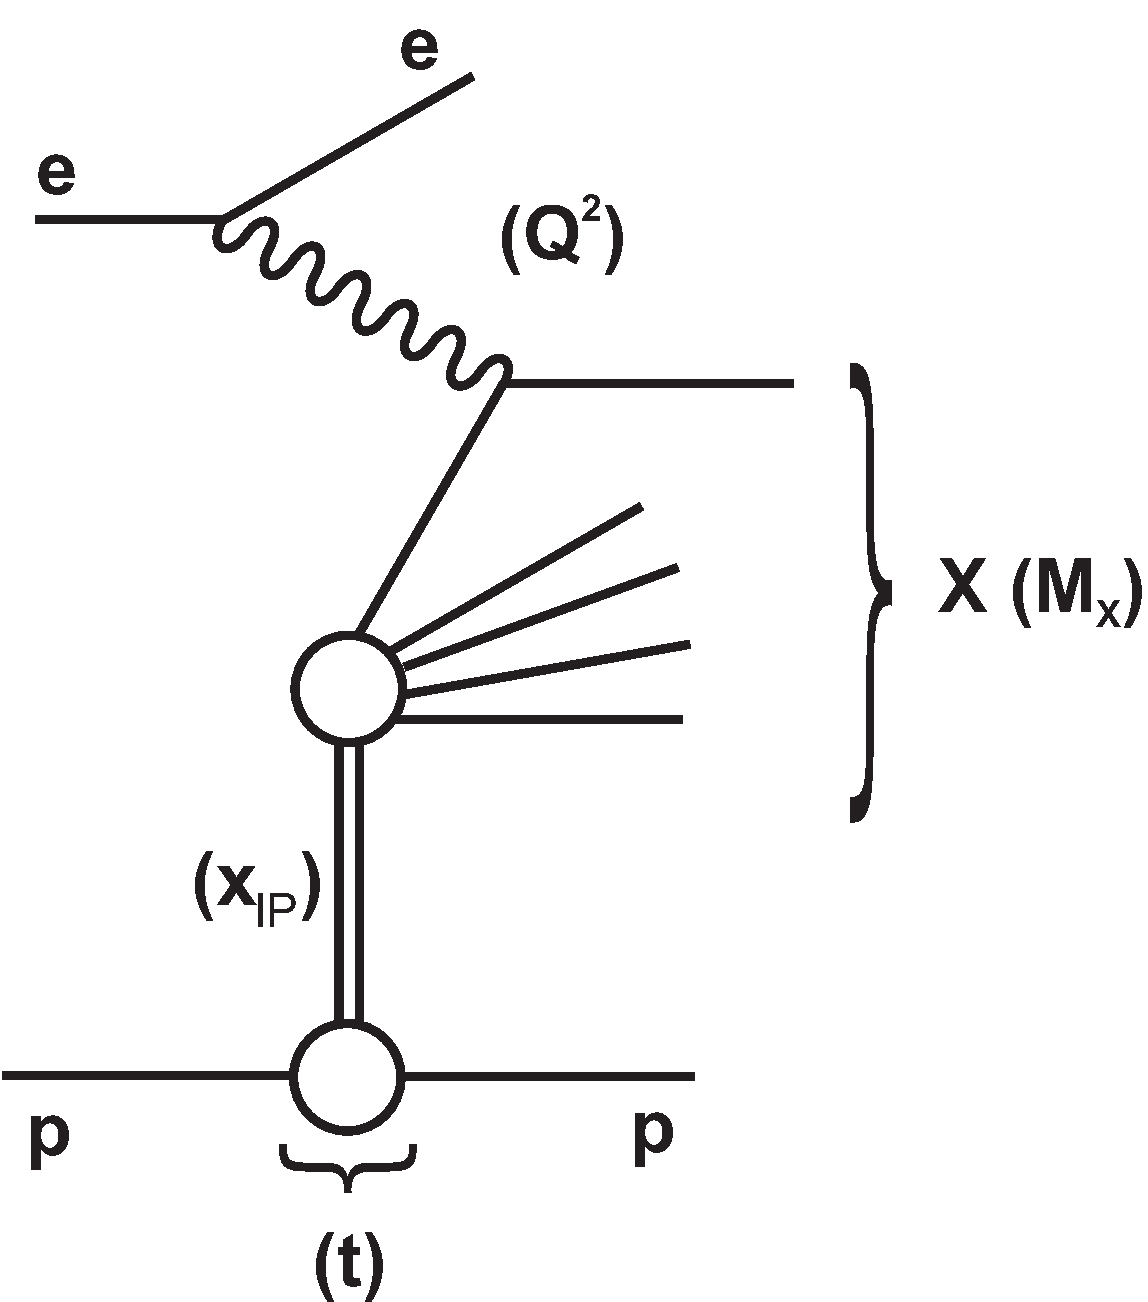
\includegraphics[width=0.5\linewidth]{figures/diffraction.pdf}
%\end{center}
%\caption{Schematic diagram of the kinematic variables used to
% describe the inclusive diffractive DIS process.}
%\label{fig:diff}
%\end{figure}

In addition to the usual variables $x$, $Q^2$, one must consider the squared four-momentum transfer $t$
(the undetected momentum transfer to the proton system) and
the mass $M_X$ of the diffractively produced final state. 
In practice, the variable $M_X$ 
is often replaced by $\beta=\frac{Q^2}{M_X^2+Q^2-t}$.
%
In models based on a factorisable Pomeron, $\beta$ may be viewed as the fraction of the
pomeron longitudinal momentum which is carried by the struck parton, $x=\beta x_{\Pom}$.
%The diffractive parton distribution functions (DPDFs) are interpreted as probabilities for 
%finding a parton with a small fraction of the proton momentum $x=\beta\Pom$

For the inclusive case, the diffractive cross-section can be expressed as:
\begin{equation}
\begin{array}{lcl}
  \frac{d\sigma}{d\beta\,dQ^2dx_{\Pom}\,dt}
=
  \frac{2\pi\alpha^2}{\beta Q^4}\,
    \left( 1 +  (1-y)^2 \right) \ensuremath{\overline\sigma}^{D(4)}(\beta,Q^2,x_{\Pom},t)
\label{Dxs}
\end{array}
\end{equation}
where the ``reduced cross-section'' , $\overline\sigma$, is defined as
\begin{equation}
\begin{array}{lcl}
\overline\sigma^{D(4)}
 = F_2^{D(4)} - \frac{y^2}{1 +  (1-y)^2}\, F_L^{D(4)}
 = F_T^{D(4)} + \frac{2(1-y)}{1 +  (1-y)^2}\, F_L^{D(4)}.
\label{eq:sigred}
\end{array}
\end{equation}
%The dimension of $F_k^{D(4)}(\beta,Q^2,x_{\Pom},t)$
%is $GeV^{-2}$ and thus quantities integrated over $t$.
%\begin{equation}
%F_k^{D(3)}(\beta,Q^2,x_{\Pom})
%\equiv
%\int_{t_{\rm min}}^{t_{\rm max}} dt
%F_k^{D(4)}(\beta,Q^2,x_{\Pom},t)
%\end{equation}
%are dimensionless. The maximum kinematically allowed value of $t$ is given by
%\begin{equation}
%t_{\rm MAX} 
%=
%-\frac{x_{\Pom}^2 m_p^2 + p_\perp^2}{1-x_{\Pom}}
%\approx 
%-\frac{x_{\Pom}^2}{1-x_{\Pom}} m_p^2
%\end{equation}
%where $m_p$ is the proton mass.
With $x = x_{\Pom}\beta$ we can relate this to the standard DIS formula.
%\begin{equation}
%\begin{array}{lcl}
%\frac{d\sigma}{d\beta\,dQ^2\,dx_{\Pom}\,dt} =
%  \frac{2\pi\alpha^2}{x\, Q^4}\,
%    \left( 1 +  (1-y)^2 \right) x_{\Pom}\ensuremath{\overline\sigma}^{D(4)}(\beta,Q^2,x_{\Pom},t)
%\end{array}
%\end{equation}
%which upon integration over $t$ reads
%\begin{equation}
%\begin{array}{lcl}
%\label{Dxs3}
%  \frac{d\sigma}{d\beta\,dQ^2\,dx_{\Pom}}
%=  
%  \frac{2\pi\alpha^2}{x Q^4}\,
%    \left( 1 +  (1-y)^2 \right) \,x_{\Pom}\ensuremath{\overline\sigma}^{D(3)}(\beta,Q^2,x_{\Pom}).
%\end{array}
%\end{equation}
%%The H1 and ZEUS data files typically contain $x_{\Pom}\ensuremath{\overline\sigma}^{D(3)}$.
The diffractive structure functions can be expressed as convolutions of the
calculable coefficient functions with diffractive quark and gluon distribution functions,
 which in general depend on all of \xpom, $Q^2$, $\beta$, $t$.
\\
%==========================================
%{\bf Regge factorization} 
%Needed? \\
The diffractive PDFs in \fitter\ are implemented following the prescription of ZEUS
publication~\cite{zeus:diff2009} and can be used to reproduce the main results.
%For a  better description of data, a contribution from a secondary Reggeon, $\Reg$, is included, hence
%\begin{equation}
%F_k^{D(4)}(\beta,Q^2,x_{\Pom},t) = 
%\sum_{\mathcal{X} =\Pom,\Reg}
%\phi_\mathcal{X}(x_{\Pom},t)\, F^\mathcal{X}_k(\beta,Q^2)
%\end{equation}
%or
%\begin{equation}
%\label{eq:FD3}
%F_k^{D(3)}(\beta,Q^2,x_{\Pom}) = 
%\sum_{\mathcal{X} =\Pom,\Reg}
%\Phi_\mathcal{X}(x_{\Pom})\, F^\mathcal{X}_k(\beta,Q^2)
%\end{equation}
%where
%\begin{equation}
%\label{eq:intFlux}
%\Phi_{\mathcal{X}}(x_{\Pom}) =
%\int\limits_{t_{\rm min}}^{t_{\rm max}} dt\, \phi_\mathcal{X}(x_{\Pom},t)
%\,.
%\end{equation}
%The fluxes are parametrized as
%\begin{subequations}
%\label{eq:flux}
%\begin{equation}
%\phi_\mathcal{X}(x_{\Pom},t) = 
%\frac {A_\mathcal{X}\, e^{b_\mathcal{X} t}} {x_{\Pom}^{2\alpha_\mathcal{X}(t) -1}}
%\end{equation}
%where
%\begin{equation}
%\alpha_\mathcal{X}(t) = \alpha_\mathcal{X}(0) + \alpha_\mathcal{X}' t
%\,.
%\end{equation}
%\end{subequations}
%The function $F^\Reg_k(\beta,Q^2)$  is taken to be that of the pion.
%
